\documentclass[../main.tex]{subfiles}
\usepackage[utf8]{inputenc}
\usepackage[T1]{fontenc}
\usepackage{graphicx}
\usepackage{longtable}
\usepackage{wrapfig}
\usepackage{rotating}
\usepackage[normalem]{ulem}
\usepackage{amsmath}
\usepackage{amssymb}
\usepackage{capt-of}
\usepackage{hyperref}
\usepackage{float}
\graphicspath{{../}}
\author{Cezary Wieczorkowski}
\date{\today}
\title{Analiza}
\hypersetup{
 pdfauthor={Cezary Wieczorkowski},
 pdftitle={Analiza},
 pdfkeywords={},
 pdfsubject={},
 pdflang={Polish}}
\begin{document}


\section{Analiza istniejącego stanowiska}
Poniższy rozdział został napisany na podstawie \hyperref[zal:1]{załącznika nr 1}.   
\subsection{Zasada działania stanowiska}
    
    \subsubsection{Opis stanowiska}
        Zestaw laboratoryjny modeluje system komunikacji oparty na 4 bitowej szynie danych. W skład zestawu wchodzą urządzenia nadawcze i odbiorcze
        podłączone do szyny danych, logika sterująca procesem wymiany danych oraz elementy interfejsu użytkownika. Na rysunku \ref{fig:szyna_schemat} 
        możemy zobaczyć płytę czołową zestawu która przedstawia jego schemat blokowy oraz interfejs użytkownika. 
        \\
        W przypadku tego stanowiska działanie wspomnianych urządzeń jest emulowane na dwóch mikrokontrolerach. W dalszej części rozdziału
        działanie zestawu zostanie opisane tak jakby było to urządzenie zbudowane z podzespołów przedstawionych na jego płycie czołowej.

        \begin{figure}[H]
            \centering
            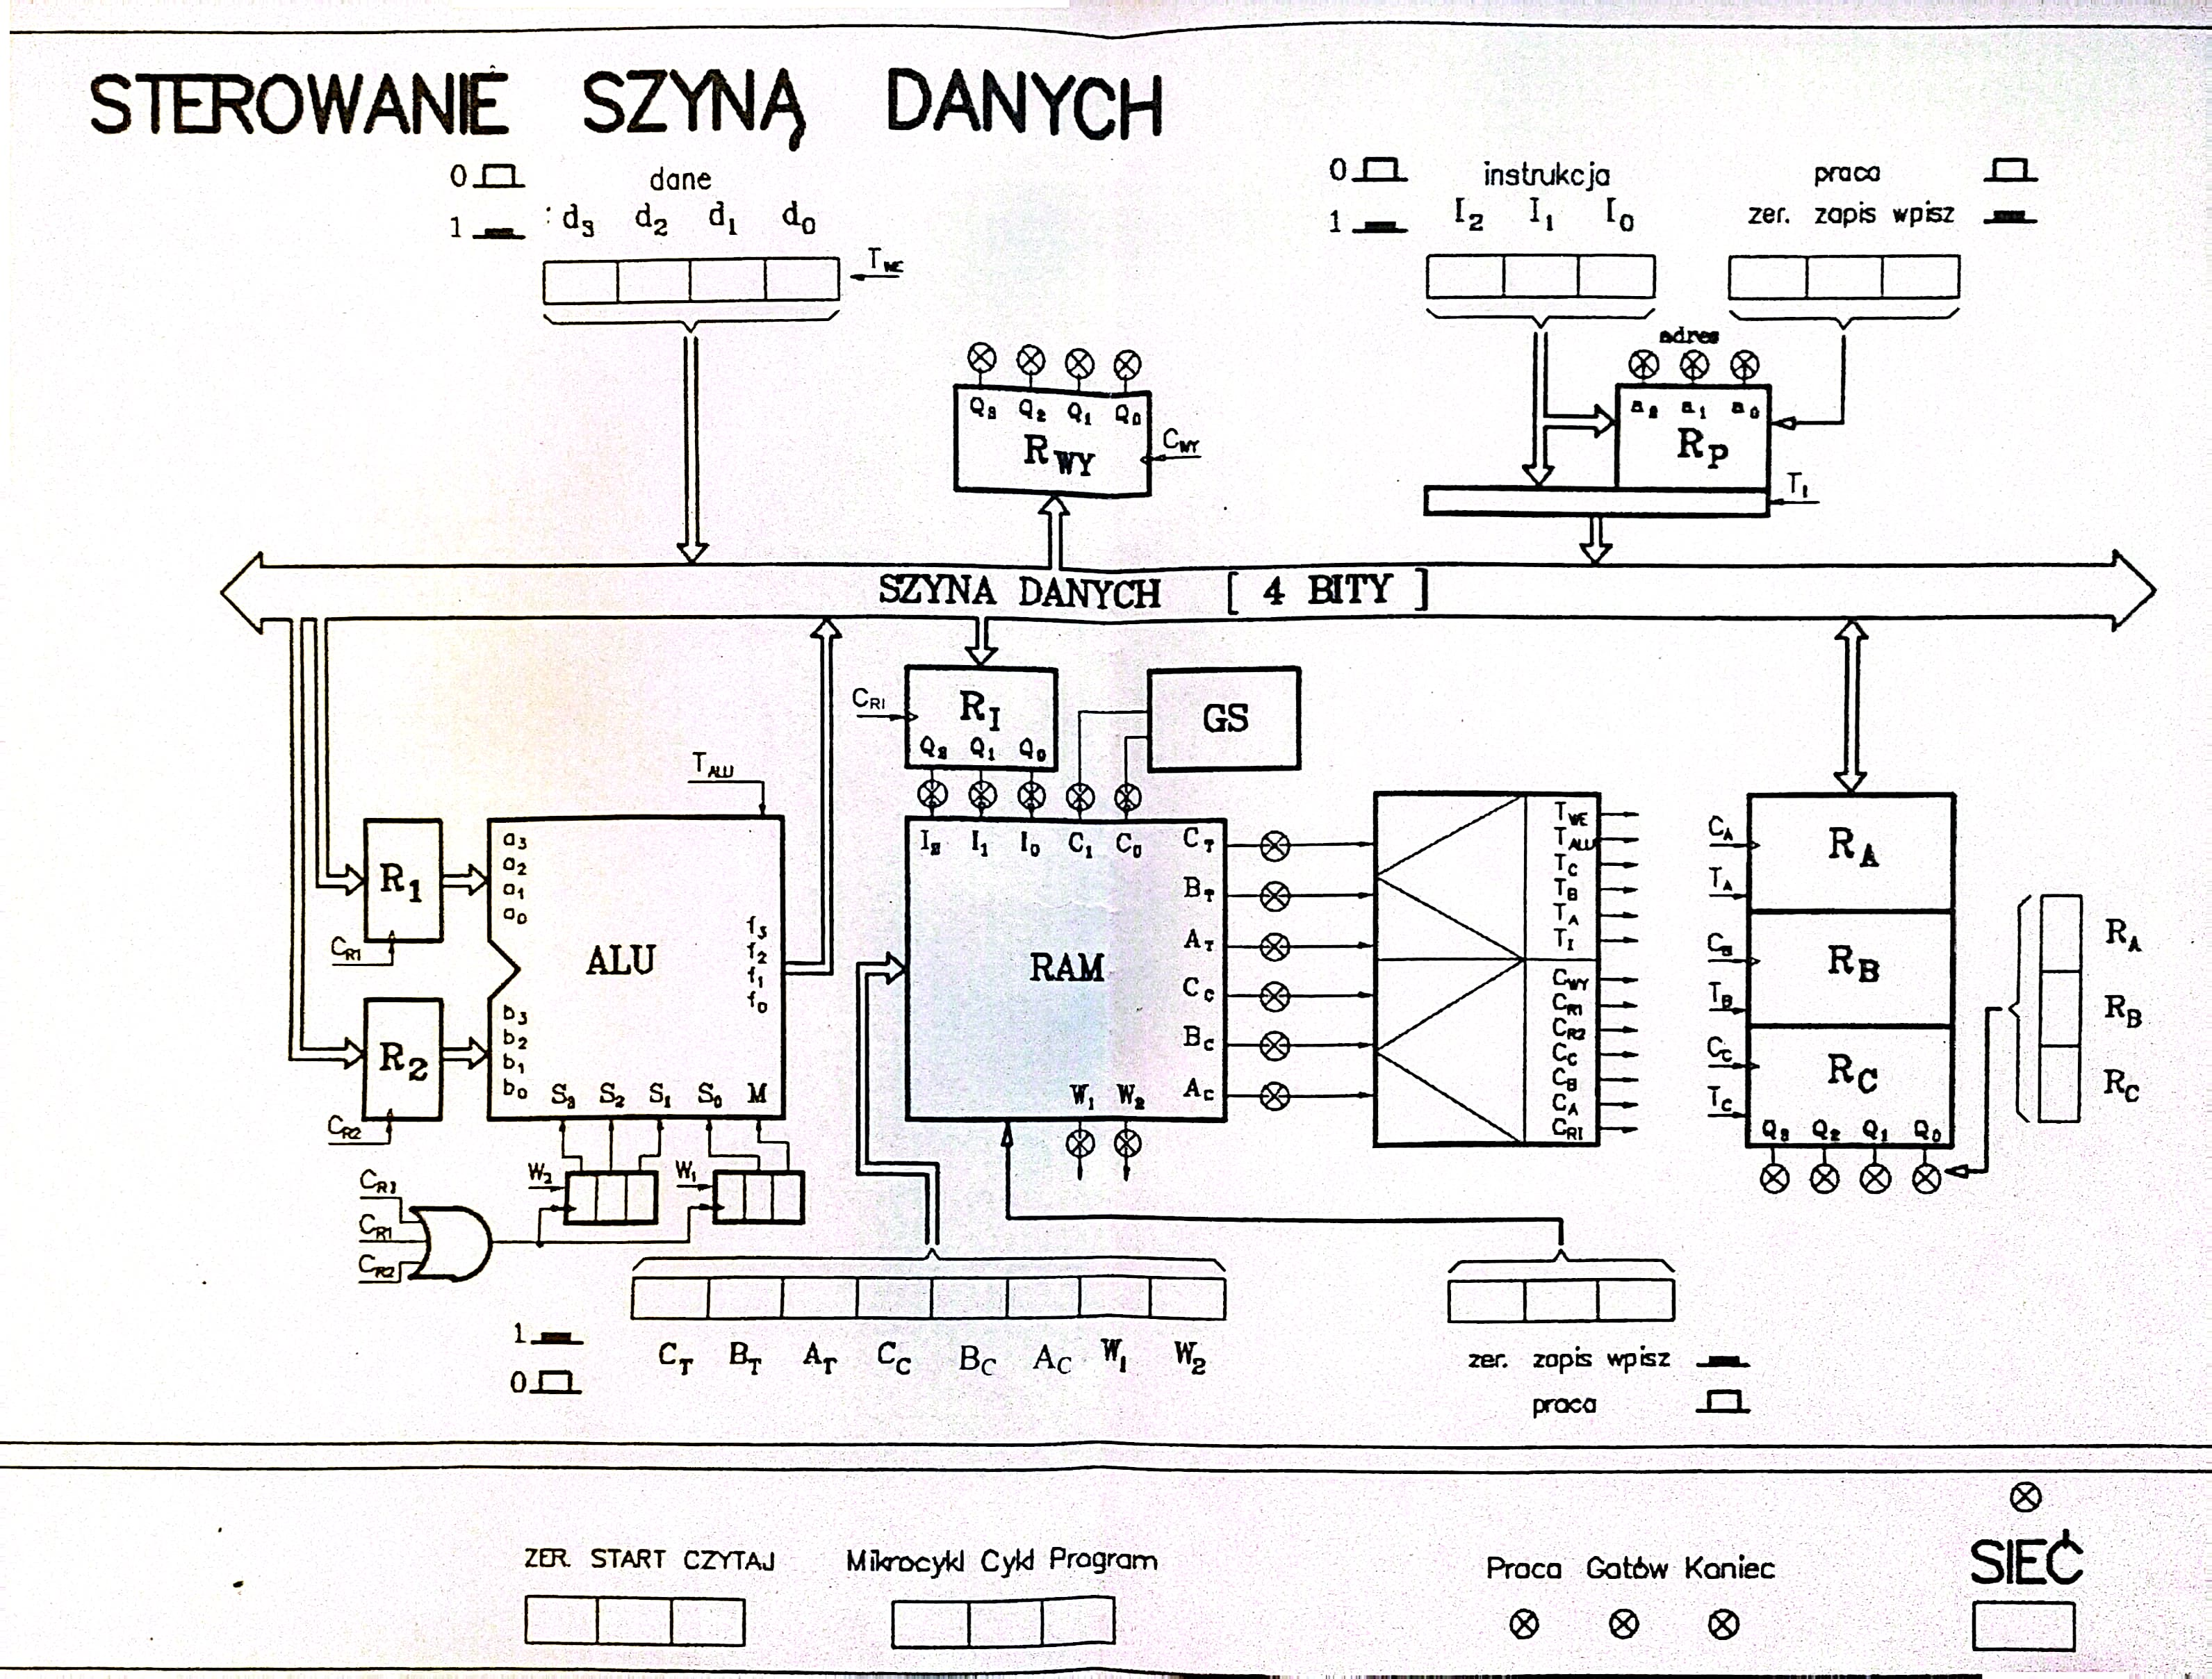
\includegraphics[width=\linewidth]{szyna_schemat.jpg}
            \caption{Płyta czołowa zestawu}
            \label{fig:szyna_schemat}
        \end{figure}

    \subsubsection{Elementy składowe stanowiska}

        \subsubsection*{Pamięć RAM}

        Pamięć ram w zestawie jest zorganizowana jako 32 słowa po 8 bitów.
        
        \begin{figure}[H]
            \centering
            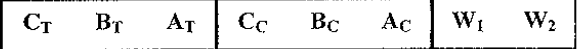
\includegraphics[width=\linewidth]{ram_symbol.png}
            \caption{Symbole przypisane  poszczególnym bitom słowa w pamięci RAM}
            \label{fig:ram_symbol}
        \end{figure}
        
        Zawartość słów w pamięci RAM kontroluję pracę zestawu:

        \begin{itemize}
            \item bity $C_T, B_T, A_T$ - wybór nadajnika na szynie
            \item bity $C_C, B_C, A_C$ - wybór odbiornika na szynie
            \item bity $W_1, W_2$ - wybór operacji ALU
        \end{itemize}

        Można więc powiedzieć że pamięć RAM zawiera instrukcje pracy zestawu. W celu wykonania kolejnych instrukcji należy zwiększyć o 1
        obecny adres pamięci. Wykonanie jednej instrukcji z pamięci RAM nazywamy mikrocyklem.
        \\
        Wejścia adresowe pamięci są połączone z rejestrem Rp (trzy najstarsze bity) oraz z generatorem Gs (dwa najmłodsze bity). 
        Trzy najstarsze bity wyjścia danych pamięci połączone są z wejściami adresowymi dekodera 1 natomiast kolejne trzy z wejściami 
        adresowymi dekodera 2. Dwa najmłodsze bity wyjścia danych pamięci połączone są wejściami informacyjnymi rejestrów przesównych instrukcji ALU.

        \subsubsection*{Generator GS}
        
        Generator GS jest licznikiem modulo 4. Jego wyjścia połączone są z dwoma najmłodszymi wejściami adresowymi pamięci RAM. Podczas pracy
        generator wygeneruje kolejno wartości dwóch najstarszych bitów adresu od 00 do 11. W zależności od trybu pracy zestawu generowane są
        kolejne adresy pamięci do zapisu lub odczytu i wykonani jako instrukcje w mikrocyklu.

        \subsubsection*{Dekoder sygnałów sterujących}
        
        Dekodery sygnałów sterujących to układy konwertujące liczby binarne na kod 1 z n. Dekoder 1 wytwarza sygnały sterujące nadajnikami które
        podawane są na wejścia sterujące przyłączaniem poszczególnych nadajników do szyny dancyh.

        \begin{figure}[H]
            \centering
            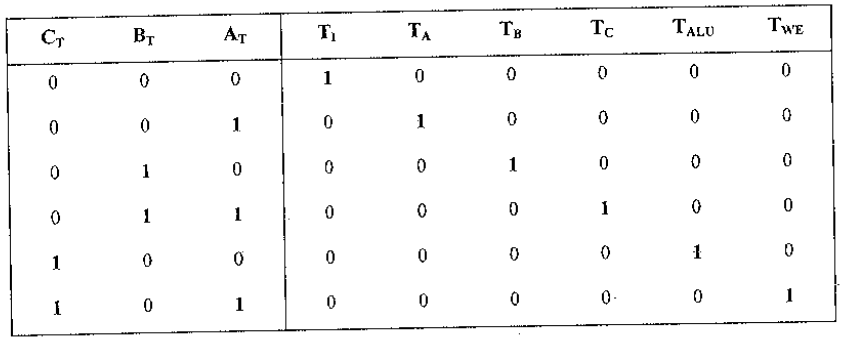
\includegraphics[width=\linewidth]{nadajniki.png}
            \caption{Tablica prawdy dla dekodera 1}
            \label{fig:nadajniki}
        \end{figure}

        Dekoder 2 działa analogicznie do dekodera 1 ale wytwarza sygnały sterujące odbiornikami. Sygnały generowane przez dekoder 1 podawane
        są na wejścia zapisu poszczególnych odbiorników.

        \begin{figure}[H]
            \centering
            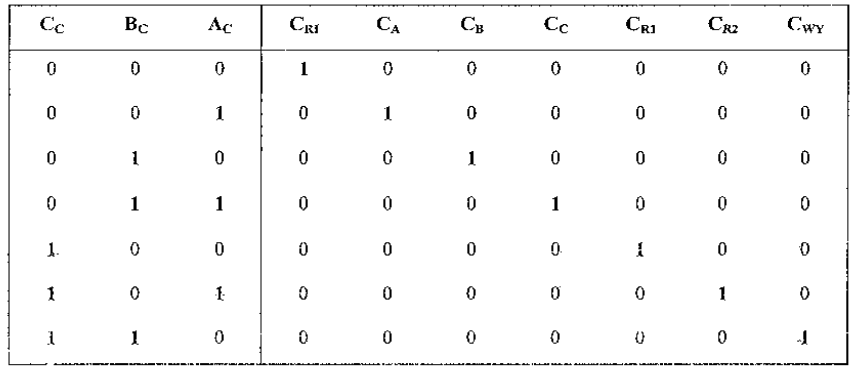
\includegraphics[width=\linewidth]{odbiorniki.png}
            \caption{Tablica prawdy dla dekodera 2}
            \label{fig:odbiorniki}
        \end{figure}

        \subsubsection*{Jednostka arytmetyczno logiczna ALU}
        
        Układ ten realizuje operacje arytmetyczne i logiczne na dwóch liczbach 4 bitowych zapisanych w rejestrach $R_1$ oraz $R_2$.
        Rodzaj wykonywanej operacji określa pięciobitowe słowo $M, S_3, S_2, S_1, S_0$ które jest zapizywane w dwóch 3 bitowych rejestrach przesównych.
        Na rysunku \ref{fig:szyna_schemat} widzimy sposób połączenia rejestrów przesównych w układzie. Na ich wejścia danych podane są 
        sygnały $W_1, W_2$ z pamięci RAM. Natomiast na wejścia zegarowe podana jest suma logiczna sygnałów $C_RI, C_R1, C_R2$. Z tych zależności
        wynika, że podczas projektowania instrukcji z użyciem ALU w celu ustawienia odpowiedniego kodu operacji należy przewidzieć 
        wygenerowanie sygnałów $C_RI, C_R1, C_R2$. Na rysunku \ref{fig:kodowanie_alu} przedstawiono sposób kodowania operacji do wykonania przez ALU.

        \begin{figure}[H]
            \centering
            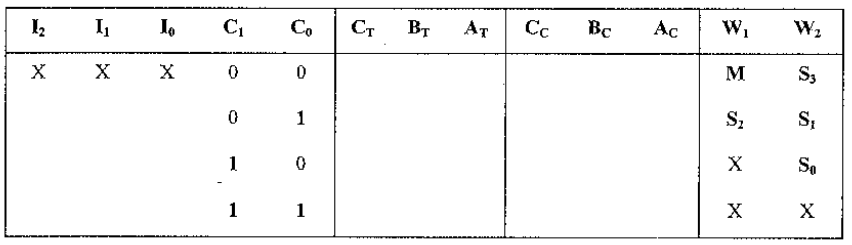
\includegraphics[width=\linewidth]{kodowanie_alu.png}
            \caption{Zasada kodowania operacji do wykonania przez ALU}
            \label{fig:kodowanie_alu}
        \end{figure}

        Jednostka arytmetyczno logiczna ma możliwość zrealizowania 16 operacji arytmetycznych oraz logicznych:

        \begin{figure}[H]
            \centering
            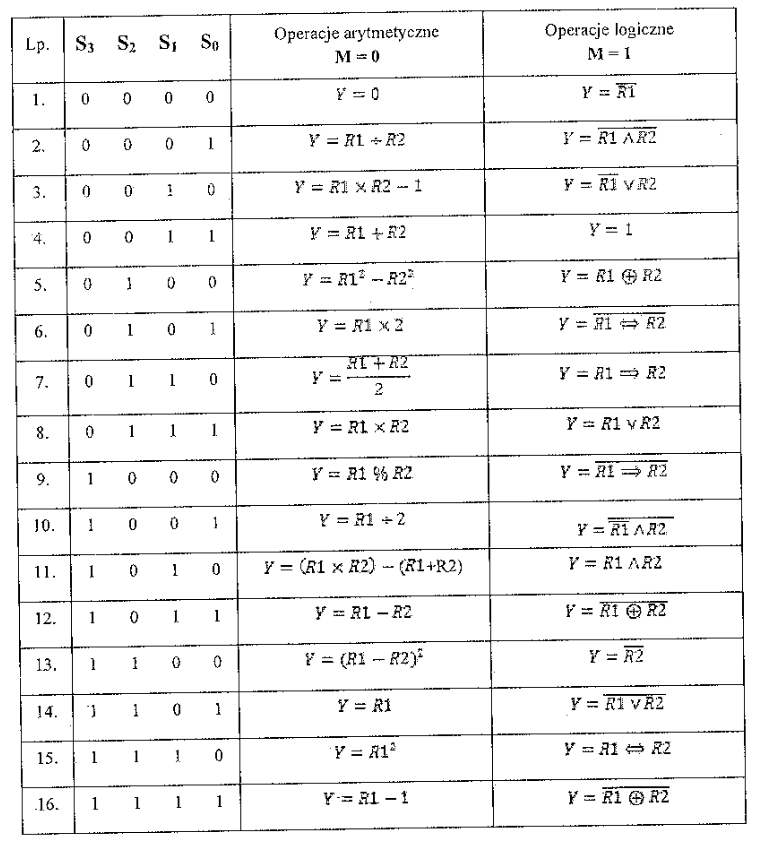
\includegraphics[width=\linewidth]{operacje_alu.png}
            \caption{Lista operacji realizowanych przez ALU}
            \label{fig:operacje_alu}
        \end{figure}

        \subsubsection*{Rejestry pomocnicze}
        Rejestry są układami przechowującymi dane. W zestawie występują następujące rejestry:
        \begin{itemize}
            \item $R_A, R_B, R_C$ - są to rejestry przeznaczone do wykorzystania przez użytkownika, 
            mogą one zarówno odbierać jak i nadawać dane na szynę
            \item $R_1 R_2$ - przechowują argumenty operacji ALU, mogą tylko odbierać dane z szyny
            \item $R_{wy}$ - służy do prezentacji wyników operacji wykonywanych przez zestaw laboratoryjny, może tylko odbierać dane z szyny
            \item $R_I$ - przechowuje trzy najstarsze bity adresu pamięci, może tylko odbierać dane z szyny
            \item $R_p$ - to zespół ośmiu rejestrów przeznaczonych do przechowywania adresów pamięci RAM pod którymi znajdują
            się instrukcje do wykonania przez zestaw. Rejestr ten jest wykorzystywany w trybie pracy Program
        \end{itemize}

    \subsubsection{Interfejs użytkownika}

    \subsubsection{Tryby pracy stanowiska}

\subsection{Krytyczna ocena stanowiska} %mabe lepszy tytuł?

    \subsubsection{Zalety stanowiska}

    \subsection{Wady stanowiska}

\end{document}